\chapter{Introduction to Numerical Integration}
\label{chap:intro-numint}
\section{Overview}
\emph{Numerical integration} seeks to approximate definite integrals when an exact analytical solution is unavailable or impractical. This is achieved by replacing the continuous integral with a weighted sum over discrete points:

\begin{equation}
\int_a^b f(x) \, dx \approx \sum_{i=1}^n w_i f(x_i)
\end{equation}

where \(x_i\) are nodes and \(w_i\) are weights determined by the chosen quadrature method (from Latin \emph{quadratura}, "making square").
Common methods include the \textbf{midpoint rule}, \textbf{trapezoidal rule}, and \textbf{Simpson's rule}, each characterized by specific error terms and convergence rates. For example, the error in the trapezoidal rule is \(\mathcal{O}((b-a)^3 f''(\xi)/n^2)\), while Simpson's rule has error \(\mathcal{O}((b-a)^5 f^{(4)}(\xi)/n^4)\) for some \(\xi \in [a,b]\).

\begin{figure}[h!]
  \centering
  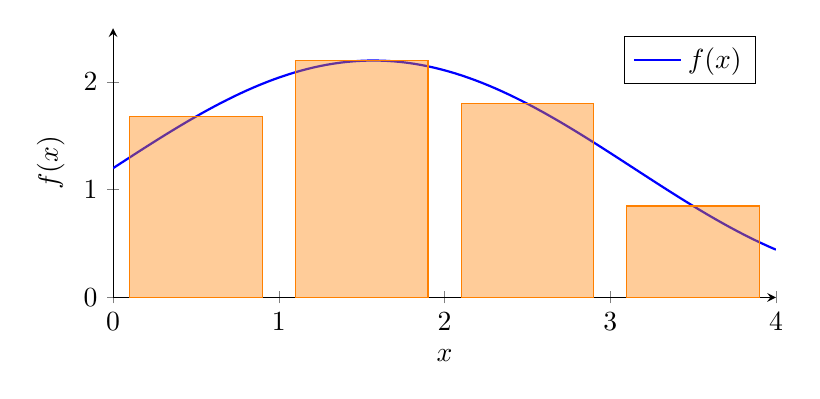
\begin{tikzpicture}
  \begin{axis}[
    width=10cm, height=5cm,
    axis x line=bottom,
    axis y line=left,
    xlabel={\(x\)},
    ylabel={\(f(x)\)},
    ymin=0, ymax=2.5,
    xmin=0, xmax=4,
    samples=100,
    domain=0:4,
    xtick={0,1,2,3,4},
    ytick={0,1,2},
    legend pos=north east
  ]
  \addplot [blue, thick] {sin(deg(x)) + 1.2};
  \addlegendentry{\(f(x)\)}
  % Draw rectangles for midpoint rule
  \foreach \i in {0,1,2,3} {
    \addplot [
    ybar,
    bar width=0.8,
    fill=orange, fill opacity=0.4,
    draw=orange
    ] coordinates {({\i+0.5},{sin(deg(\i+0.5))+1.2})};
  }
  \end{axis}
  \end{tikzpicture}
  \caption{Illustration of estimating the area under the curve \(f(x)\) using the midpoint rule. The orange rectangles represent the approximation. This figure shows how the area under the curve \(f(x)\) can be estimated by summing the areas of the orange rectangles.}
  \label{fig:numint-midpoint}
\end{figure}

In this part, we will systematically develop the theory and practical aspects of numerical integration, with emphasis on:

\begin{itemize}
  \item \textbf{Integration Methods:} Detailed introduction to the midpoint, trapezoidal, and Simpson's rules for approximating definite integrals, i.e., \(I \approx \int_a^b f(x) \, dx\). We will discuss the construction, application, and comparative advantages of each method.
  \item \textbf{Error Analysis:} Examination of error bounds and convergence rates, typically expressed as \(\mathcal{O}(h^p)\) for step size \(h\) and method order \(p\). We will also address stability criteria for quadrature rules, such as the requirement \(\sum_i |w_i| < C\) for some constant \(C\), and clarify the meaning of convergence (\(I_h \to I\) as \(h \to 0\)).
\end{itemize}

\section{Fundamental Principles}

We consider numerical methods to compute:
\begin{equation}
    I(f) = \int_a^b f(x) \, dx
\end{equation}

Any explicit formula to approximate $I(f)$ is called a \textbf{quadrature formula} or \textbf{numerical integration formula}.

\subsection{General Principle}

The general approach consists of:
\begin{enumerate}
    \item Construct an explicitly integrable function $f_n$, $n \geq 0$, to approximate $f$ on $[a,b]$ (e.g., by interpolation)
    \item Define $I_n(f) = I(f_n)$
\end{enumerate}

For $f \in C([a,b])$, the quadrature error $E_n(f) = I(f) - I_n(f)$ satisfies:
\begin{equation}
    |E_n(f)| = \left|\int_a^b [f(x) - f_n(x)] \, dx\right| \leq \int_a^b |f(x) - f_n(x)| \, dx \leq \max_{x \in [a,b]} |f(x) - f_n(x)| \cdot (b-a)
\end{equation}

\section{Interpolatory Quadrature Formulas}

\subsection{Basic Construction}

Take $f_n = \Pi_n f$, i.e., the interpolation polynomial to $f$ with respect to some nodes $\{x_0, \ldots, x_n\}$, since this is easily integrable. Then:
\begin{equation}
    f_n = \sum_{i=0}^n f(x_i) \ell_i(x), \quad \ell_i(x) = \prod_{\substack{k=0\\k \neq i}}^n \frac{x - x_k}{x_i - x_k} \in \mathbb{P}_n
\end{equation}

and we get:
\begin{equation}
    I_n(f) = I(f_n) = \int_a^b f_n(x) \, dx = \sum_{i=0}^n \left(\int_a^b \ell_i(x) \, dx\right) f(x_i)
\end{equation}

The coefficients $\alpha_i = \int_a^b \ell_i(x) \, dx$ are independent of $f$. They just depend on the nodes $\{x_0, \ldots, x_n\}$!

This is an instance of a \textbf{linear formula}:
\begin{equation}
    I_n(f) = \sum_{i=0}^n \alpha_i f(x_i)
\end{equation}

\subsection{Extended Linear Formulas and Exactness}

We can extend a linear formula to include derivatives $f^{(q)}(x_i)$, $q = 0, \ldots, Q$:
\begin{equation}
    I_n(f) = \sum_{i=0}^n \sum_{q=0}^Q \alpha_{iq} f^{(q)}(x_i)
\end{equation}
for example using Hermite interpolation ($Q = 1$), where $\alpha_{iq} \in \mathbb{R}$.

\begin{definition}{Degree of Exactness}{degree-exactness}
The \textbf{degree of exactness} of a quadrature formula is the maximum integer $r$ such that:
\[I_n(f) = I(f) \text{ for all } f \in \mathbb{P}_r\]
\end{definition}

\section{Classical Quadrature Rules}

The midpoint, trapezoidal, and Simpson rules are fundamental examples. We assume these are known, including analysis of their errors:

\begin{itemize}
    \item \textbf{Midpoint rule}: $\int_a^b f(x) \, dx \approx (b-a) f\left(\frac{a+b}{2}\right)$
    \item \textbf{Trapezoidal rule}: $\int_a^b f(x) \, dx \approx \frac{b-a}{2}[f(a) + f(b)]$
    \item \textbf{Simpson rule}: $\int_a^b f(x) \, dx \approx \frac{b-a}{6}\left[f(a) + 4f\left(\frac{a+b}{2}\right) + f(b)\right]$
\end{itemize}

Please review these fundamental rules and refresh your memory.

\section{Newton-Cotes Formulas}

Newton-Cotes formulas are based on interpolation with the special case of equispaced points in $[a,b]$:
\[x_k = x_0 + kh, \quad k = 0, \ldots, n\]

These include the midpoint, trapezoidal, and Simpson rules.

A formula is called:
\begin{itemize}
    \item \textbf{closed} if $x_0 = a$ and $x_n = b$, and we obtain $h = \frac{b-a}{n}$, $n \geq 1$
    \item \textbf{open} if $x_0 = a + h$ and $x_n = b - h$, and we have $h = \frac{b-a}{n+2}$, $n \geq 0$
\end{itemize}

Then:
\begin{itemize}
    \item Midpoint rule is the open formula with $n = 0$
    \item Trapezoidal and Simpson are the closed formulas for $n = 1, 2$, respectively
\end{itemize}

\subsection{Newton-Cotes Properties}

The weights $\alpha_i$ in the linear formula $I_n(f) = \sum_{i=0}^n \alpha_i f(x_i)$ with equispaced $x_i$ depend only on $n$ and $h$.

We obtain with $\phi_i(t) = \prod_{\substack{k=0\\k \neq i}}^n \frac{t-k}{i-k}$:

\begin{itemize}
    \item \textbf{closed}: $I_n(f) = h \sum_{i=0}^n w_i f(x_i)$, $w_i = \int_0^n \phi_i(t) \, dt$
    \item \textbf{open}: $I_n(f) = h \sum_{i=0}^n w_i f(x_i)$, $w_i = \int_{-1}^{n+1} \phi_i(t) \, dt$
\end{itemize}

Key properties:
\begin{itemize}
    \item $h$ only appears as a factor in front
    \item $n$ determines the number of coefficients/summands and appears once in every weight $w_i$
    \item $\Rightarrow$ precompute and store
\end{itemize}

\subsection{Precomputed Newton-Cotes Weights}

\begin{itemize}
    \item In the closed formulas: by symmetry of $\phi_i$ and $\phi_{n-i}$ $\Rightarrow w_i = w_{n-i}$ for $i = 0, \ldots, n-1$ for even $n$
    \item For odd cases, similarly: $w_i = w_{n-i}$, $i = 0, \ldots, n$
    \item We only have to store $w_i$, $i < \frac{n+1}{2}$
    \item Higher order open NC formulas: negative weights
\end{itemize}
\subsubsection{Closed Newton-Cotes Weights}

\begin{center}
\begin{tabular}{|c|c|c|c|}
\hline
$n$ & Formula Name & Weights $w_i$ & Degree of Exactness \\
\hline
1 & Trapezoidal & $w_0 = w_1 = \frac{1}{2}$ & 1 \\
\hline
2 & Simpson's & $w_0 = w_2 = \frac{1}{6}$, $w_1 = \frac{4}{6}$ & 3 \\
\hline
3 & Simpson's 3/8 & $w_0 = w_3 = \frac{1}{8}$, $w_1 = w_2 = \frac{3}{8}$ & 3 \\
\hline
4 & Boole's & $w_0 = w_4 = \frac{7}{90}$, $w_1 = w_3 = \frac{32}{90}$, $w_2 = \frac{12}{90}$ & 5 \\
\hline
\end{tabular}
\end{center}

\subsubsection{Open Newton-Cotes Weights}

\begin{center}
\begin{tabular}{|c|c|c|c|}
\hline
$n$ & Formula Name & Weights $w_i$ & Degree of Exactness \\
\hline
0 & Midpoint & $w_0 = 2$ & 1 \\
\hline
1 & Two-point & $w_0 = w_1 = \frac{3}{2}$ & 1 \\
\hline
2 & Three-point & $w_0 = w_2 = \frac{4}{3}$, $w_1 = \frac{2}{3}$ & 3 \\
\hline
3 & Four-point & $w_0 = w_3 = \frac{5}{4}$, $w_1 = w_2 = \frac{3}{4}$ & 3 \\
\hline
\end{tabular}
\end{center}

\textbf{Note:} For $n \geq 8$ in closed formulas and $n \geq 3$ in open formulas, some weights become negative, which can lead to numerical instability.

\subsection{Error Analysis for Newton-Cotes Formulas}

\begin{theorem}{Newton-Cotes Error}{nc-error}
Let $f \in C^{(n+2)}([a,b])$ and $n > 1$ be given. The error $E_n(f) = I(f) - I_n(f)$ reads:

For even $n$:
\[E_n(f) = \frac{M_n}{(n+2)!} h^{n+3} f^{(n+2)}(\xi)\]

For odd $n$:
\[E_n(f) = \frac{K_n}{(n+1)!} h^{n+2} f^{(n+1)}(\xi)\]

for some $\xi \in (a,b)$, where using $\pi_{n+1}(t) = \prod_{i=0}^n (t-i)$ we have:

\begin{align}
M_n &= \begin{cases}
\int_0^n t\pi_{n+1}(t) \, dt & \text{for closed} \\
\int_{-1}^{n+1} t\pi_{n+1}(t) \, dt & \text{for open}
\end{cases} \\
K_n &= \begin{cases}
\int_0^n \pi_{n+1}(t) \, dt & \text{for closed} \\
\int_{-1}^{n+1} \pi_{n+1}(t) \, dt & \text{for open}
\end{cases}
\end{align}
\end{theorem}

\section{Composite Newton-Cotes Formulas}

\subsection{Motivation}

\begin{enumerate}
    \item Avoid high polynomial degree (i.e., on large intervals $[a,b]$ or "complicated" $f$)
    \item Known: composite Midpoint | Trapezoidal | Simpson rule
\end{enumerate}

\subsection{The Idea}

Write $[a,b]$ as $m$ subintervals:
\[\int_a^b f(x) \, dx = \sum_{j=0}^{m-1} \int_{T_j} f(x) \, dx\]

with $T_j = [y_j, y_{j+1}]$, $y_j = a + jH$, $j = 0, \ldots, m$, i.e., $H = \frac{b-a}{m}$

$\Rightarrow$ Perform Newton-Cotes on each $T_j$ (of length $H$) with (equispaced) nodes $x_k^{(j)}$ and weights (computed earlier) $\alpha_k^{(j)}$, $0 \leq k \leq n$, to obtain:
\[I_{n,m}(f) = \sum_{j=0}^{m-1} \sum_{k=0}^n \alpha_k^{(j)} f(x_k^{(j)})\]

\subsection{Composite Newton-Cotes Error}

\begin{theorem}{Composite Newton-Cotes Error}{composite-nc-error}
Let $f \in C^{(n+2)}(a,b)$, $m$ be given and $n$ be even. Then:
\[E_{n,m}(f) = I(f) - I_{n,m}(f) = \frac{b-a}{(n+2)!} M_n H^{n+2} f^{(n+2)}(\xi)\]

and for odd $n$:
\[E_{n,m}(f) = I(f) - I_{n,m}(f) = \frac{b-a}{(n+1)!} K_n \frac{\gamma_n H^{n+1}}{\gamma_{n+2}} f^{(n+1)}(\xi)\]

for some $\xi \in (a,b)$, where:
\begin{itemize}
    \item $M_n$ and $K_n$ are as before
    \item $\gamma_n = \begin{cases} n+2 & \text{for open} \\ n & \text{for closed} \end{cases}$ formulas
\end{itemize}
\end{theorem}

\section{Richardson Extrapolation for Numerical Integration}

\subsection{Basic Idea}

Small step sizes give good results. Extrapolate on $h$.

Suppose a numerical method depends smoothly on a step size $h$, e.g., $h = \frac{b-a}{n}$:
\[Q(h) = I_n(f) = I(f) + \alpha_1 h + \alpha_2 h^2 + \alpha_3 h^3 + \ldots\]

\textbf{Idea II:} Evaluate $Q$ for different values of $h$, for example $h$ and $\delta h$, $\delta < 1$. Typically: $\delta = \frac{1}{2}$.

\begin{align}
Q(h) &= I(f) + \alpha_1 h + \alpha_2 h^2 + \alpha_3 h^3 + \ldots \\
Q(\delta h) &= I(f) + \alpha_1 \delta h + \alpha_2 \delta^2 h^2 + \alpha_3 \delta^3 h^3 + \ldots
\end{align}

\textbf{Goal:} Eliminate the first error term $\alpha_1 h$ by computing:
\[Q(\delta h) - \delta Q(h) = (1-\delta) I(f) + 0 + \alpha_2 \delta (\delta - 1) h^2 + (\cdots) h^3 + \ldots\]

\subsection{Richardson Extrapolation Formula}

We divide the equation by $1-\delta$ and obtain:
\[\tilde{Q}(h) := \frac{Q(\delta h) - \delta Q(h)}{1-\delta} = I(f) - \alpha_2 \delta h^2 + (\cdots) h^3 + \ldots\]
\[= I(f) + \tilde{\alpha}_2 h^2 + \tilde{\alpha}_3 h^3 + \ldots, \quad \tilde{\alpha}_k = \frac{\delta^k - \delta}{1-\delta} \alpha_k\]

Observe that:
\begin{itemize}
    \item We took our "old"/original scheme $Q(h)$ and evaluated it twice (for $h$ and $\delta h$)
    \item We obtain an explicit formula for $\tilde{Q}$
    \item $\Rightarrow$ since $h$ is small, the largest error term vanishes $\Rightarrow$ more accurate!
    \item We obtain a higher order method (at least accurate up to 2nd order)
\end{itemize}

\subsection{Iterative Richardson Extrapolation}

But even more: If we have:
\begin{itemize}
    \item $\tilde{Q}(h)$ (based on $Q(h)$ and $Q(\delta h)$)
    \item $\tilde{Q}(\delta h)$ (based on $Q(\delta h)$ and $Q(\delta^2 h)$)
\end{itemize}

$\Rightarrow$ Build $\hat{Q}(h)$ from these two to eliminate the $h^2$ term!

This iteration process is called \textbf{Richardson extrapolation}.

Note that there exist methods with only even powers of $h$ in their expansion, i.e.:
\[Q(h) = I(f) + \alpha_2 h^2 + \alpha_4 h^4 + \alpha_6 h^6 + \ldots\]

Then the scheme is even faster in obtaining accuracy, order would increase by 2 in every step!

\section{Euler-Maclaurin Summation Formula}

Let $f \in C^{2k+2}([a,b])$. We approximate $I(f) = \int_a^b f(x) \, dx$ by a composite trapezoidal rule.

Let $T_m$ be the composite trapezoidal rule with $h = h_m = \frac{b-a}{m}$, i.e.:
\[T_m(f) = \frac{1}{2} h_m f(a) + h_m \sum_{j=1}^{m-1} f(a + jh_m) + \frac{1}{2} h_m f(b)\]

Then one can prove:
\[T_m(f) = I(f) + \sum_{i=1}^k \frac{B_{2i}}{(2i)!} h_m^{2i} [f^{(2i-1)}(b) - f^{(2i-1)}(a)] + R_{2k+2}\]

where:
\begin{itemize}
    \item remainder $R_{2k+2} = \frac{B_{2k+2}}{(2k+2)!} (b-a) f^{(2k+2)}(\eta)$ for some $\eta \in (a,b)$
    \item Bernoulli numbers $B_j$ are given by the generating (power) series (or Taylor series at $z = 0$):
    \[\frac{z}{e^z - 1} = \sum_{k=0}^{\infty} \frac{B_k}{k!} z^k\]
    and $B_{2k+1} = 0$, $k > 0$
\end{itemize}

\section{Romberg Integration}

Named after Werner Romberg (1909-2003), this method employs the extrapolation procedure with $\delta = \frac{1}{2}$.

Here we use $h_m = \frac{b-a}{2^m}$ and we use the trapezoidal rule initially:
\[A_{m,0} = T_{2^m}(f) = \frac{1}{2} h_m f(a) + h_m \sum_{j=1}^{2^m-1} f(a + jh_m) + \frac{1}{2} h_m f(b), \quad m = 0,1,\ldots\]

Hence we get from Euler-Maclaurin:
\[A_{m,0} = I(f) + \sum_{i=1}^{\infty} \alpha_i h_m^{2i} \quad \text{and} \quad A_{m-1,0} = I(f) + \sum_{i=1}^{\infty} \alpha_i h_{m-1}^{2i} = \sum_{i=1}^{\infty} \alpha_i 2^{2i} h_m^{2i}\]

$\Rightarrow$ For $2^2 A_{m,0} = 2^2 I(f) + \sum_{i=1}^{\infty} \alpha_i 2^2 h_m^{2i}$ the terms for $i = 1$ agree. Hence:
\[2^2 A_{m,0} - A_{m-1,0} = (2^2 - 1) I(f) + \sum_{i=2}^{\infty} \beta_i h_m^{2i} \text{ for some } \beta_i\]

Define:
\[A_{m,1} := \frac{2^2 A_{m,0} - A_{m-1,0}}{2^2 - 1} = I(f) + \sum_{i=2}^{\infty} \tilde{\alpha}_i h_m^{2i}\]

\subsection{General Romberg Formula}

By induction for $q \geq 0$:
\[A_{m,q+1} = \frac{4^{q+1} A_{m,q} - A_{m-1,q}}{4^{q+1} - 1} = I(f) + \sum_{i=q+2}^{\infty} \alpha_{i,q+1} h_m^{2i}\]

\subsection{Romberg Integration Table}

We start with $A_{0,0}$ and $A_{1,0}$, i.e., (composite) trapezoidal rules with $h_0 = b-a$ and $h_1 = \frac{b-a}{2}$.

Similarly you can compute $A_{m,0}$, $m = 2,3,\ldots$ by a trapezoidal rule.

We continue with the scheme:
\[
\begin{array}{cccccc}
A_{0,0} \\
A_{1,0} & A_{1,1} \\
A_{2,0} & A_{2,1} & A_{2,2} \\
A_{3,0} & A_{3,1} & A_{3,2} & A_{3,3} \\
\vdots  & \vdots  & \vdots  & \vdots  & \ddots
\end{array}
\]

Overall we have the error $A_{m,n} = I(f) + O(h_m^{2(n+1)})$.

\subsection{Why Dyadic Steps?}

Recall:
\[A_{m,0} = T_{2^m}(f) = \frac{1}{2} h_m f(a) + h_m \sum_{j=1}^{2^m-1} f(a + jh_m) + \frac{1}{2} h_m f(b)\]

but we also have using $h_{m-1} = 2h_m$ that:
\[\frac{1}{2} A_{m-1,0} = T_{2^{m-1}}(f) = \frac{1}{2} h_m f(a) + h_m \sum_{j=1}^{2^{m-1}-1} f(a + 2jh_m) + \frac{1}{2} h_m f(b)\]

So subtracting them yields:
\[A_{m,0} - \frac{1}{2} A_{m-1,0} = h_m \sum_{r=1}^{2^{m-1}} f(a + (2r-1)h_m) = \frac{1}{2} U_{2^{m-1}}\]

Where $U_{2^{m-1}}$ is the midpoint rule on the new points, or:

The dyadic scheme lets us compute $A_{m,0} = \frac{1}{2}(A_{m-1,0} + U_{2^{m-1}})$, where the midpoint rule is computed only with the new points.

\section{Improper Integrals}

\subsection{Computing Integrals - Overview}
\begin{enumerate}
  \item Jump discontinuity at $c \in [a,b]$ $\Rightarrow$ split: $\int_a^b f(x) \, dx = \int_a^c f(x) \, dx + \int_c^b f(x) \, dx$ $\Rightarrow$ easy!
  \item The case where $f(x)$ is unbounded, i.e., if $\lim_{x \to a^+} f(x) = \pm\infty$ (analogously $\lim_{x \to b^-} f(x) = \pm\infty$)
  \item The case where $a$ is unbounded, i.e.,
  \[
    \lim_{a \to -\infty} \int_a^b f(x) \, dx = \int_{-\infty}^b f(x) \, dx
    \quad \text{analogously, } \lim_{b \to \infty} \int_a^b f(x) \, dx = \int_a^{\infty} f(x) \, dx
  \]
  If both appear, use idea from 1.
\end{enumerate}

\subsection{Integrals with Infinite Functions}

Not all of them exist, for example $\int_0^{\infty} \frac{1}{x} \, dx$ has no finite value.

Compare to $\int_0^1 \frac{1}{2\sqrt{x}} \, dx$ $\Rightarrow$ the integral exists, antiderivative is $\sqrt{x}$.

We consider the special case where $f$ is of the form (model):
\[f(x) = \frac{\phi(x)}{(x-a)^{\mu}}, \quad 0 \leq \mu < 1\]

where $\phi(x)$ is bounded on $[a,b]$ and we need $\phi$ to be smooth, i.e., $\phi \in C^{p+1}([a,b])$. Let's denote the bound by $|\phi(x)| \leq M$ for $x \in [a,b]$.

Then we can obtain plausibility:
\[\int_a^b f(x) \, dx \leq M \int_a^b \frac{1}{(x-a)^{\mu}} \, dx = M \frac{1}{1-\mu} (x-a)^{1-\mu} \Big|_a^b = M \frac{(b-a)^{1-\mu}}{1-\mu}\]

\subsection{Ansatz for this Model of Functions}

For any $0 < \varepsilon < 1$ (and $a + \varepsilon < b$) we split:
\[I(f) = I_1 + I_2 = \int_a^{a+\varepsilon} \frac{\phi(x)}{(x-a)^{\mu}} \, dx + \int_{a+\varepsilon}^b \frac{\phi(x)}{(x-a)^{\mu}} \, dx\]

where:
\begin{itemize}
    \item we can compute $I_2$ with methods we already know
    \item in $I_1$ we can use ($\phi$ smooth!) the Taylor expansion of $\phi$:
\end{itemize}

\[\phi(x) = \Phi_p(x) + R_{p+1} = \sum_{k=0}^p \frac{1}{k!} \phi^{(k)}(a)(x-a)^k + \frac{(x-a)^{p+1}}{(p+1)!} \phi^{(p+1)}(\xi(x))\]

where $\xi(x) \in (a,x)$.

And obtain for:
\[f(x) = \frac{\Phi_p(x)}{(x-a)^{\mu}} + \frac{R_{p+1}(x)}{(x-a)^{\mu}} = \sum_{k=0}^p \frac{\phi^{(k)}(a)}{k!} (x-a)^{k-\mu} + \frac{(x-a)^{p+1-\mu}}{(p+1)!} \phi^{(p+1)}(\xi(x))\]

\subsection{Solving the Integral \texorpdfstring{$I_1$}{I1}}

The function $f$ of the form above can now be integrated (on $[a, a+\varepsilon]$), they are just monomials. We get:
\[I_1 = \varepsilon^{1-\mu} \sum_{k=0}^p \frac{\phi^{(k)}(a)}{k!(k+1-\mu)} \varepsilon^k + \frac{1}{(p+1)!} \int_a^{a+\varepsilon} (x-a)^{p+1-\mu} \phi^{(p+1)}(\xi(x)) \, dx\]
\[=: I_{1,p} + R_{1,p+1}\]

We obtained an expression for $I_1$ where:
\begin{itemize}
    \item we can compute $I_{1,p}$
    \item but we have to get an idea about the error $|R_{1,p+1}|$ we make
\end{itemize}

\subsection{Error Bound for \texorpdfstring{$|R_{1,p+1}|$}{R1,p+1}}

To bound:
\[R_{1,p+1} = \frac{1}{(p+1)!} \int_a^{a+\varepsilon} (x-a)^{p+1-\mu} \phi^{(p+1)}(\xi(x)) \, dx\]

Idea: Replace/bound $\phi^{(p+1)}(\xi(x))$ by $C_{\varepsilon} = \max_{a \leq x \leq a+\varepsilon} |\phi^{(p+1)}(x)|$.

Then:
\[E_1 = |R_{1,p+1}| \leq \frac{1}{(p+1)!} C_{\varepsilon} \int_a^{a+\varepsilon} (x-a)^{p+1-\mu} \, dx = \frac{\varepsilon^{p+2-\mu}}{(p+1)!(p+2-\mu)} C_{\varepsilon}\]

Note: The error bound is an increasing function in $\varepsilon$.

\subsection{Back to the Complete Integral}

For $I_2$ on $[a+\varepsilon, b]$ we can use any composite Newton-Cotes formula. Here we use:
\begin{itemize}
    \item $m$ subintervals, $h = \frac{b-a-\varepsilon}{m}$
    \item composite trapezoidal rule $T_n = \frac{h}{2} f(a+\varepsilon) + \sum_{j=1}^{n-1} f(a+\varepsilon+jh) + \frac{h}{2} f(b)$
\end{itemize}

We obtain an additional error (cf. QSS (9.12) and (9.26), or as a special case of Thm. 9.3):
\[E_T = -\frac{h^2(b-a-\varepsilon)|f''(\eta)|}{12}, \quad \eta \in (a+\varepsilon, b)\]

Goal: Choose $\varepsilon$ and $p$ such that the overall behavior:
\begin{itemize}
    \item obtain a certain accuracy
    \item balance between $E_1$ and $E_T$
\end{itemize}

\subsection{Unbounded Intervals}

We again split:
\[\int_a^{\infty} f(x) \, dx = \int_a^c f(x) \, dx + \int_c^{\infty} f(x) \, dx = I_1 + I_2\]

\paragraph{Method 1:}
\begin{itemize}
    \item find a bound for the second integral $I_2$
    \item set $c$ large enough such that we can omit the value of $I_2$
    \item use any method for the first term $I_1$
\end{itemize}

\paragraph{Method 2:}
Define $t = \frac{1}{x}$ and do a change of variable:
\[I_2 = \int_c^{\infty} f(x) \, dx = \int_0^{1/c} t^{-2} f\left(\frac{1}{t}\right) \, dt = \int_0^{1/c} g(t) \, dt\]

for $g(t) = t^{-2} f\left(\frac{1}{t}\right)$ $\Rightarrow$ Solve that instead.

Note: $g(t)$ may be singular at $t = 0$, use Method from case 2.

\paragraph{Method 3:}
Gaussian Quadrature (next topic).

\begin{example}{Exam 2001, Problem 3 b/c}{exam-2001-example}
Compute:
\[I = \int_0^{\infty} \frac{e^{-x}}{1+x} \, dx = \int_0^A \frac{e^{-x}}{1+x} \, dx + \int_A^{\infty} \frac{e^{-x}}{1+x} \, dx = I_1 + I_2\]

by Method 1 using the composite trapezoidal rule $T(h)$ with step size $h$ for the integral $I_1$.

1. Prove that there exist upper bounds for:
   \[|I_1 - T(h)| \leq E_1(A,h) = \frac{5}{12} Ah^2 \quad \text{and} \quad I_2 \leq E_2(A) = e^{-A}\]

2. Approximate the integral $I$ to an error of $\varepsilon = 10^{-3}$ with as few as possible evaluations of the integrand (i.e., smallest $n$) in the trapezoidal rule ($h = \frac{A}{n}$).
\end{example}
